\chapter{Results}

\section{Simulated results}
This section lists the results from the simulation done in the Keysight Advanced Design System (ADS) software suite.

\subsection{Transistor I-V curve}

  \begin{figure}[H]
	  \centering
	  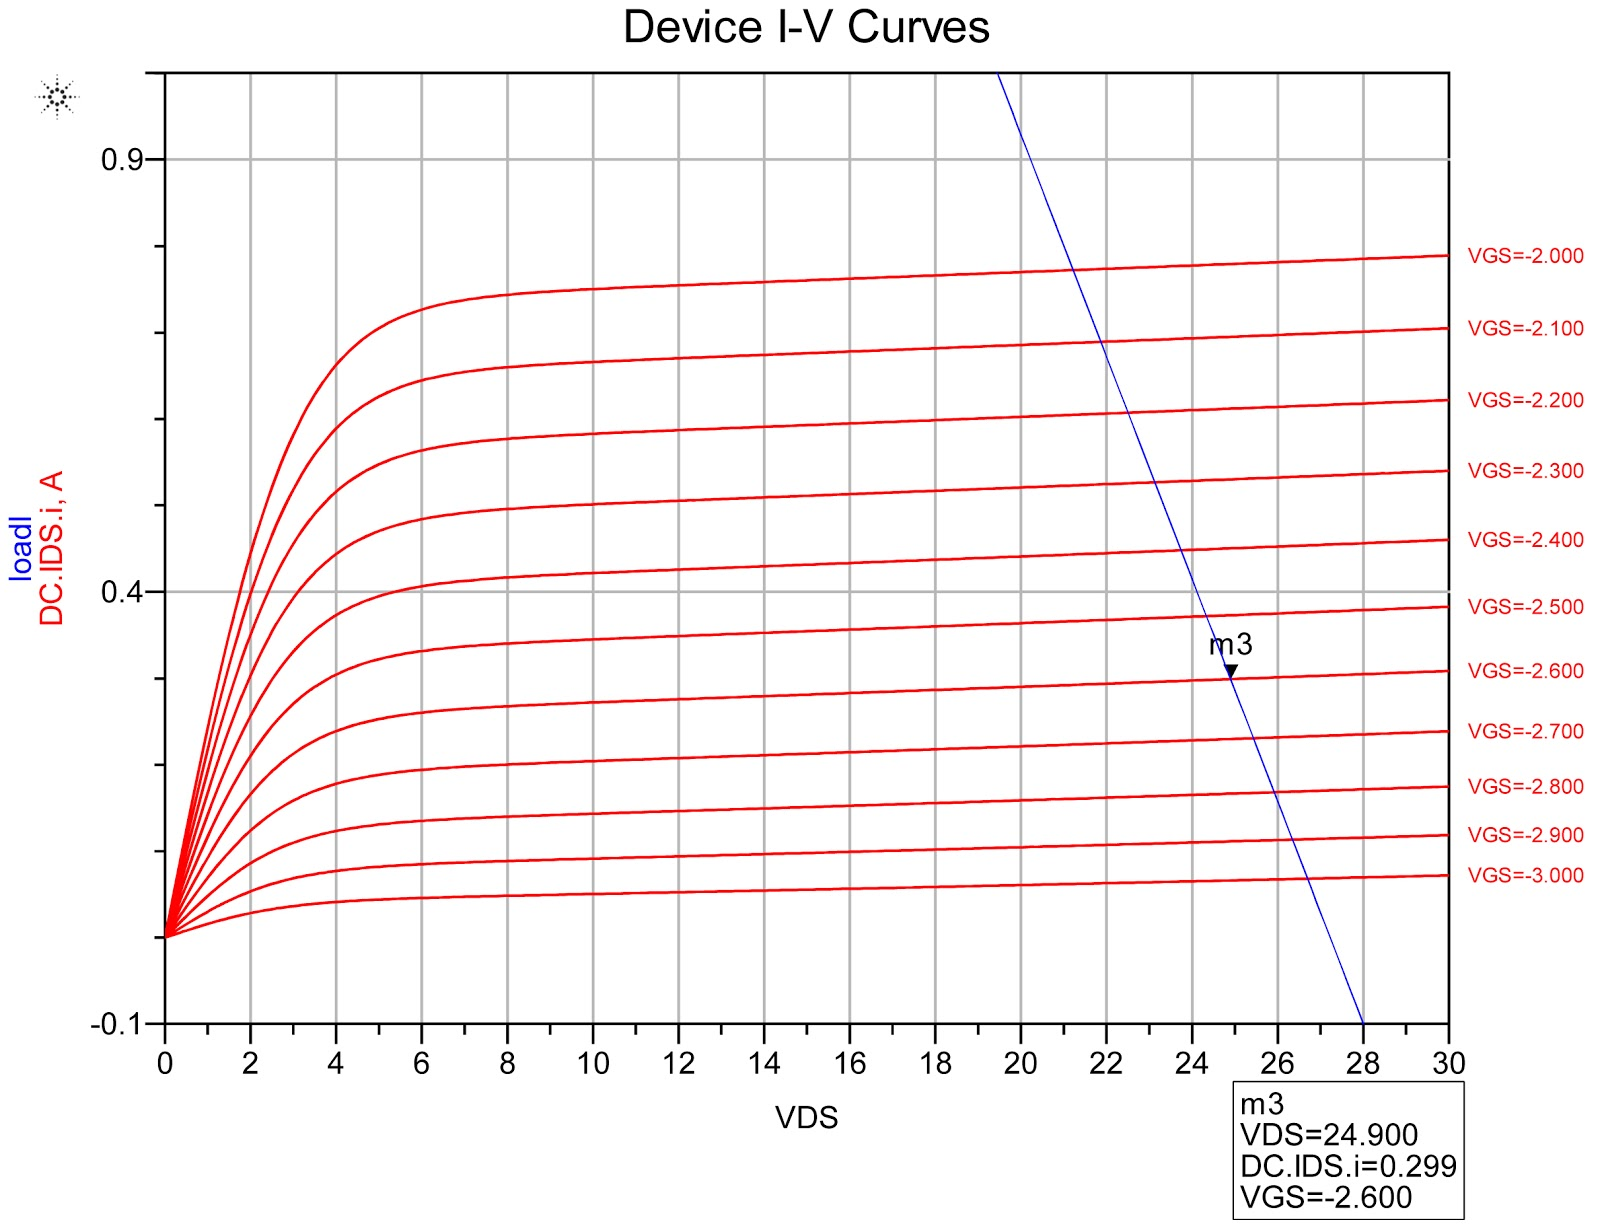
\includegraphics[width=0.75\textwidth]{img/01_IVCurve}
	  \caption{Simulated drain current for different drain and gate bias voltages with a load-line}
	  \label{fig:fig_IV}
  \end{figure}

  Note that the transistor model used is only valid for VDS voltages between 28 and 48 volts, meaning that the I-V-curves are at best approximate below 28 volts.

  \subsection{Stability simulations}

  \begin{figure}[H]
	  \begin{minipage}[b]{.45\textwidth}
	  \centering
	  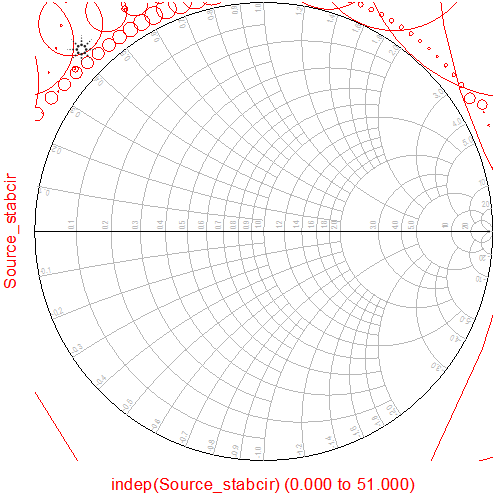
\includegraphics[width=\linewidth]{img/Stabilization_source_circle}
  	  %\caption{Amplifier input stability circle}
	  \label{fig:Stabcircle_in}
  \end{minipage}%
  \begin{minipage}{.1\textwidth}
	  \hspace{\linewidth}
  \end{minipage}%
  \begin{minipage}[b]{.45\textwidth}
	  \centering
	  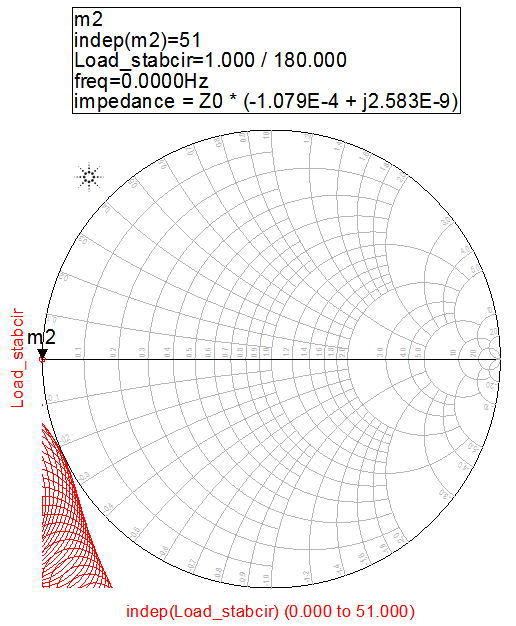
\includegraphics[width=\linewidth]{img/Stabilization_load_circle}
  	  %\caption{Amplifier output stability circle}
	  \label{fig:Stabcircle_out}
  \end{minipage}
  \caption{Smith-chart representation of the stability circles for source (left) and load (right) for frequencies between 0Hz and 6GHz}
  \label{fig:Stabcircle}
  \end{figure}

  \subsection{Small-signal gain}

  \begin{figure}[H]
	  \centering
	  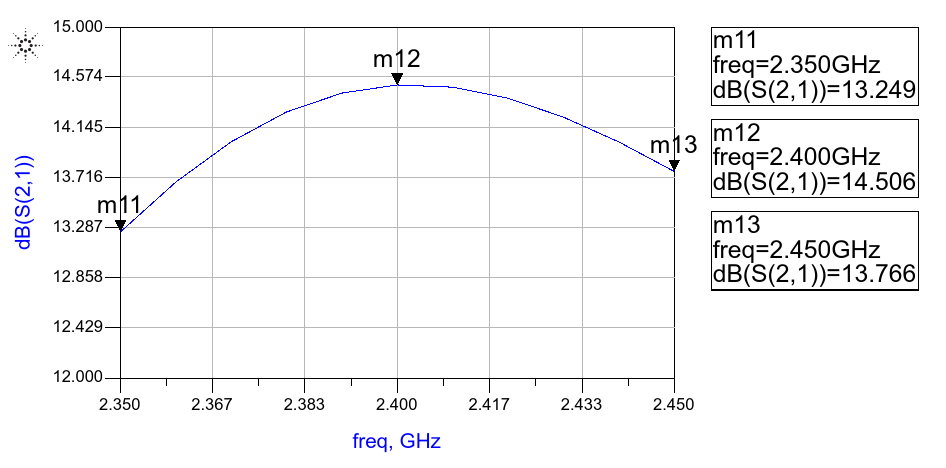
\includegraphics[width=0.75\textwidth]{img/Sim_S21}
	  \caption{Simulated small-signal gain within the band of operation}
	  \label{fig:Sim_S21}
  \end{figure}

  The small-signal gain ($S_{21}$) has a peak value of 14.506 dB at 2.4GHz, and a minimum value within the band of operations of 13.287 dB, giving a maximum variation of 1.257 dB within the 100MHz band of operation.

  \subsection{Large-signal gain}

  \begin{table}[H]
	  \centering
	  \begin{tabular}{l l l}
		  Frequency & Output power & gain \\
		  2.35 GHz & 38.71dBm & 11.71dB \\
		  2.40 GHz & 39.26dBm & 12.26dB \\
		  2.45 GHz & 38.87dBm & 11.87dB
	  \end{tabular}
	  \caption{Simulated output power with input power of 27dBm}
	  \label{tab:sim_power}
  \end{table}

  \subsection{Power added efficiency (PAE)}
  
  \begin{table}[H]
	  \centering
	  \begin{tabular}{l l}
		  Frequency & PAE \\
		  2.35 GHz & 40.30\% \\
		  2.40 GHz & 41.79\% \\
		  2.45 GHz & 42.59\%
	  \end{tabular}
	  \caption{Simulated power added efficiency with output power of 38dBm}
	  \label{tab:sim_pae}
  \end{table}

  \subsection{Third-order intermodulation distortion (TOIMD)}

  \begin{table}[H]
	  \centering
	  \begin{tabular}{l l}
		  TOIMD high & -15.35dBc \\
		  TOIMD low & -15.62dBc
	  \end{tabular}
	  \caption{Simulated third-order intermodulation distortion with output power of 38dBm}
	  \label{tab:sim_toimd}
  \end{table}

  \section{Measured results}
  This section lists the results from the measurements done on the real circuit in the laboratory.

  \subsection{Small-signal gain}

  \begin{figure}[H]
	  \centering
	  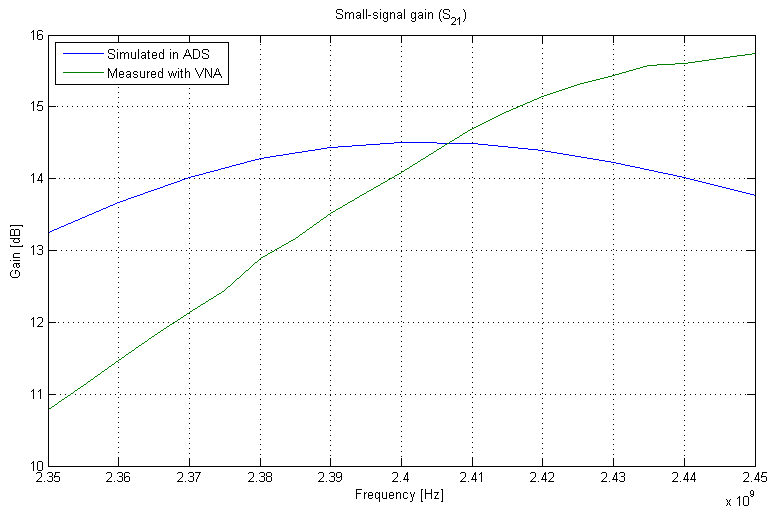
\includegraphics[width=0.75\textwidth]{img/S21_meas_sim}
	  \caption{Measured small-signal gain (green) compared to simulated small-signal gain (blue) within the band of operation}
	  \label{fig:Meas_S21}
  \end{figure}

Minimum measured gain was 10.79dB at 2.35 GHz, while the maximum was measured to 15.74dB at 2.45 GHz. At the center frequency of 2.40 GHz the small-signal gain was 14.08dB

  \subsection{Large-signal gain}

  \begin{figure}[H]
	  \centering
	  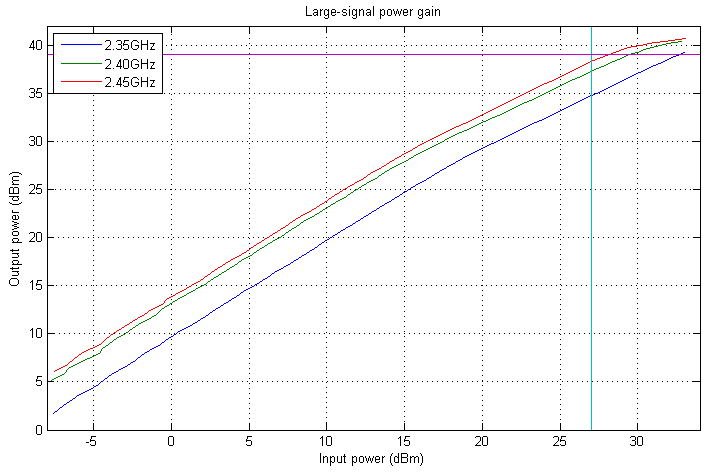
\includegraphics[width=0.75\textwidth]{img/Power_Out_1tone}
	  \caption{Measured output power at three different frequencies}
	  \label{fig:Meas_Pout}
  \end{figure}

  \begin{table}[H]
	  \centering
	  \begin{tabular}{l l l}
		  Frequency & Output power\\
		  2.35 GHz & 34.73dBm \\
		  2.40 GHz & 37.17dBm \\
		  2.45 GHz & 38.37dBm
	  \end{tabular}
	  \caption{Measured power output with an input power of 27dBm}
	  \label{tab:Meas_Pout}
  \end{table}

  \subsection{Power added efficiency (PAE)}

  \begin{figure}[H]
	  \centering
	  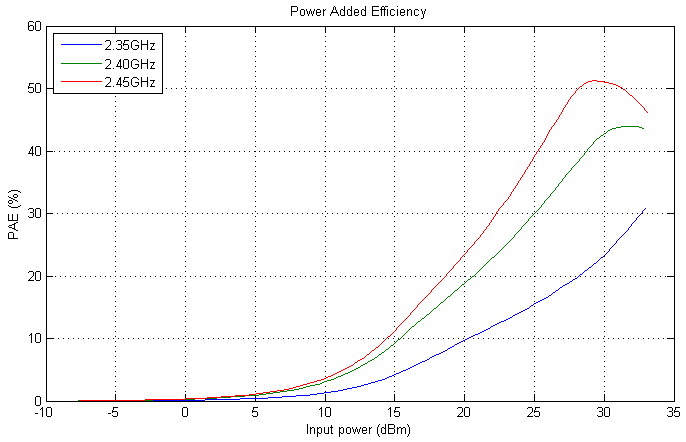
\includegraphics[width=0.75\textwidth]{img/Power_Added_Efficiency}
	  \caption{Measured power added efficiency at three different frequencies}
	  \label{fig:Meas_Pae}
  \end{figure}

  \begin{table}[H]
	  \centering
	  \begin{tabular}{l l}
		  Frequency & PAE \\
		  2.35 GHz & 18.26\% \\
		  2.40 GHz & 35.02\% \\
		  2.45 GHz & 46.99\%
	  \end{tabular}
	  \caption{Measured power added efficiency with output power of 38dBm}
	  \label{tab:Meas_Pae}
  \end{table}

  \subsection{Third-order intermodulation distortion}

    \begin{table}[H]
	  \centering
	  \begin{tabular}{l l}
		  TOIMD high & -22.41dBc \\
		  TOIMD low & -22.45dBc
	  \end{tabular}
	  \caption{Measured third-order intermodulation distortion with output power of 38dBm}
	  \label{tab:Meas_Toimd}
  \end{table}

  \subsection{Summary of measured results}

  \begin{table}[H]
	  \centering
	  \begin{tabular}{p{4.5cm} | p{1.7cm} p{2.7cm} p{1.7cm} l}
		  Parameter & 2.35 GHz & 2.40 GHz & 2.45 GHz & Requirement \\
		  \hline
		  Small-signal gain & 10.79dB & 14.08dB & 15.74dB & $>13dB$ \\
		  Output power with 27dBm input & 34.73dBm & 37.17dBm & 38.37dBm & $>39dBm$ \\
		  Power added efficiency & 18.26\% & 35.02\% & 46.99\% & - \\
		  Third-order intermodulation distortion & & high: -22.41dBc low: -22.45dBc & & - \\
	  \end{tabular}
	  \caption{Summary of measured results}
	  \label{tab:Meas_Sum}
  \end{table}


    
